\documentclass{beamer}

\mode<presentation> {
%\usetheme{default}
% \usetheme{AnnArbor}
%\usetheme{Antibes}
%\usetheme{Bergen}
%\usetheme{Berkeley}
\usetheme{Berlin}
%\usetheme{Boadilla}
%\usetheme{CambridgeUS}
%\usetheme{Copenhagen}
%\usetheme{Darmstadt}
%\usetheme{Dresden}
%\usetheme{Frankfurt}
%\usetheme{Goettingen}
%\usetheme{Hannover}
%\usetheme{Ilmenau}
%\usetheme{JuanLesPins}
%\usetheme{Luebeck}
% \usetheme{Madrid}
%\usetheme{Malmoe}
%\usetheme{Marburg}
%\usetheme{Montpellier}
%\usetheme{PaloAlto}
%\usetheme{Pittsburgh}
%\usetheme{Rochester}
%\usetheme{Singapore}
%\usetheme{Szeged}
% \usetheme{Warsaw}

%\usecolortheme{albatross}
\usecolortheme{beaver}
%\usecolortheme{beetle}
%\usecolortheme{crane}
%\usecolortheme{dolphin}
%\usecolortheme{dove}
%\usecolortheme{fly}
%\usecolortheme{lily}
%\usecolortheme{orchid}
%\usecolortheme{rose}
%\usecolortheme{seagull}
%\usecolortheme{seahorse}
%\usecolortheme{whale}
%\usecolortheme{wolverine}

\setbeamertemplate{footline} % To remove the footer line in all slides
%\setbeamertemplate{footline}[page number] % To replace the footer line in all slides
%\setbeamertemplate{navigation symbols}{} % remove the navigation symbols from the bottom of slides
}

\usepackage{graphicx}
\usepackage{booktabs}
\usepackage{bm}
\usepackage[lined,boxed]{algorithm2e}
\usepackage{hyperref}

\newcommand{\iter}[2]{#1^{(#2)}}
\DeclareMathOperator*{\argmin}{arg\,min}
\DeclareMathOperator*{\argmax}{arg\,max}


%====================================================================================
%=======================================================================   TITLE PAGE
%====================================================================================
\title[Online MM]{MM Concepts in Online Learning}
\author{Josh Day}
\institute[NC State University]{NC State University \\ \textit{jtday2@ncsu.edu}}
\date{\today}

\begin{document}

\begin{frame}
\titlepage
\end{frame}

% \begin{frame}
% \frametitle{Overview}
% \tableofcontents
% \end{frame}

%%%%%%%%%%%%%%%%%%%%%%%%%%%%%%%%%%%%%%%%%%%%%%%%%%%%%%%%%%%%%%%%%%%%%%%%%%%%%%%%%%%%% Intro
\section{Introduction}
%------------------------------------------------ Motivation
\subsection{Motivation}
\begin{frame}
  \begin{figure}
    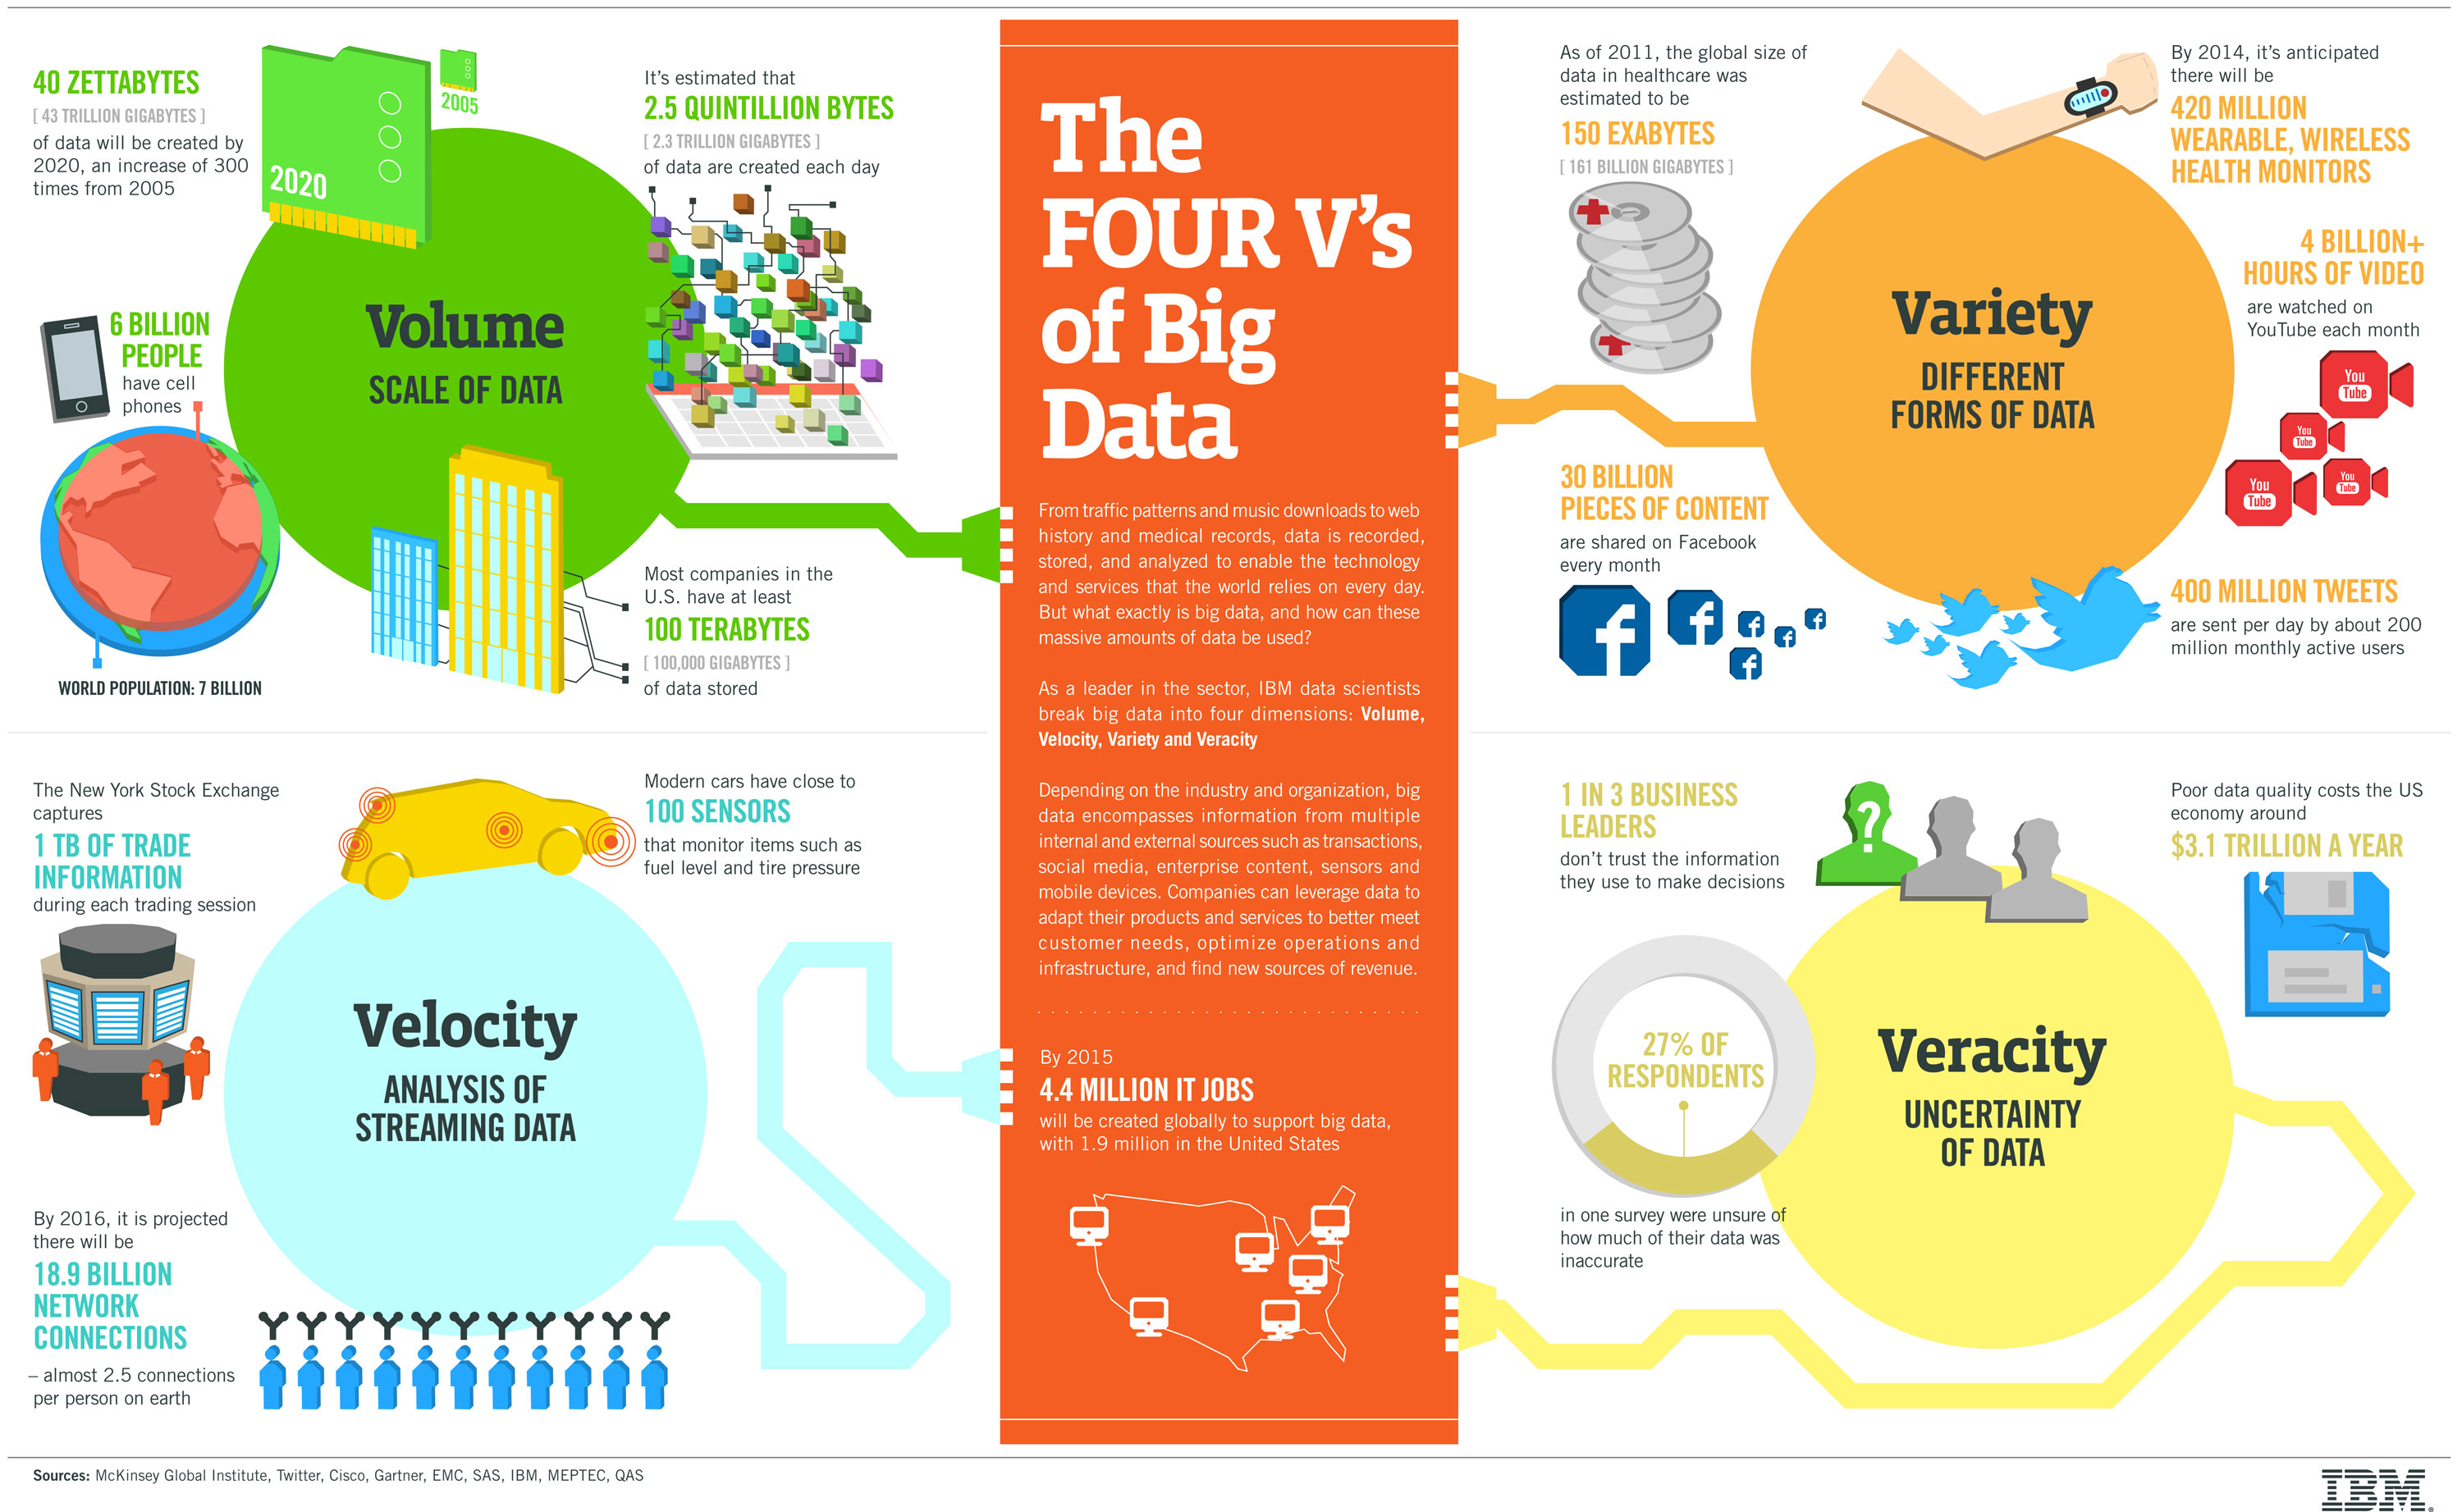
\includegraphics[width=\linewidth]{figures/4vs.jpg}
  \end{figure}
\end{frame}
\begin{frame}
  \begin{itemize}
    \item Statisticians don't have the tools to handle all of this
    \item Adapting our favorite algorithms is often nontrivial
    \item Note: If we can handle Velocity, we can handle Volume
  \end{itemize}
\end{frame}

%------------------------------------------------ What is MM
\subsection{MM Algorithms}
\begin{frame}
  \frametitle{What is an MM Algorithm?}
  \begin{itemize}
    \item MM stands for \emph{Majorization-Minimization}
    \item Solve several easy problems vs. one hard problem
    \item $h$ is said to \emph{majorize}  $f$ at $\iter{\bm\theta}{t}$ if:
    $$\begin{aligned}
      h(\bm\theta|\iter{\bm\theta}{t}) &\ge f(\bm\theta|\iter{\bm\theta}{t}) \\
      h(\iter{\bm\theta}{t}|\iter{\bm\theta}{t}) &= f(\iter{\bm\theta}{t}|\iter{\bm\theta}{t})
    \end{aligned}$$
    \item MM update: $\bm\theta^{(t+1)} = \argmin_{\bm\theta} \; h(\bm\theta|\bm\theta^{(t)})$
  \end{itemize}
\end{frame}
\begin{frame}
  \begin{figure}
    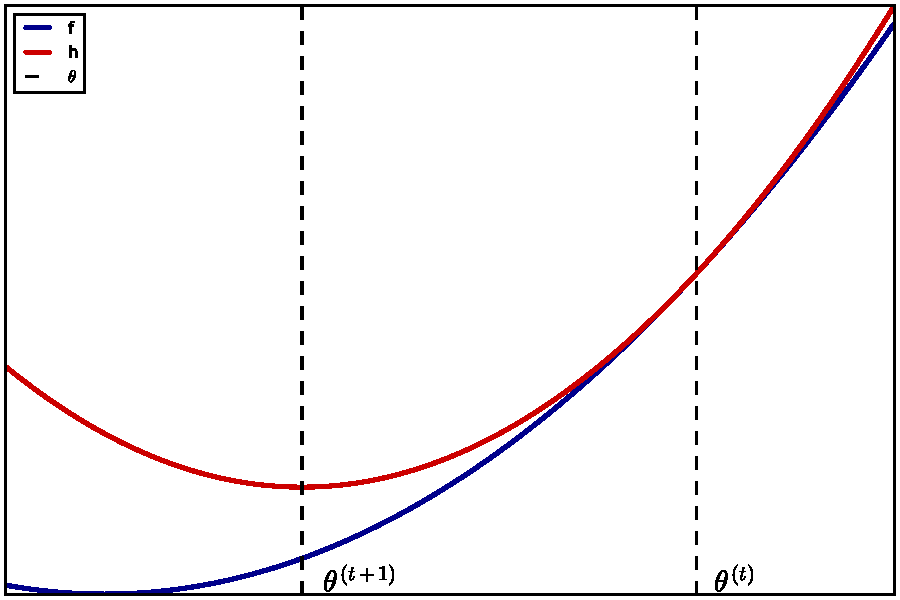
\includegraphics[width=\linewidth]{figures/mmvis.pdf}
  \end{figure}
\end{frame}
\begin{frame}
  \frametitle{Online Algorithms}
  Velocity can be handled by \emph{online algorithms}
  \begin{itemize}
    \item Entire dataset is not available at once
    \item Input enters piece by piece
    \item A well known example: Stochastic Gradient Descent
    $$\iter{\bm\theta}{t} = \iter{\bm\theta}{t-1} - \gamma_t \nabla f_t(\iter{\bm\theta}{t-1})$$
  \end{itemize}
\end{frame}
\begin{frame}
  \begin{itemize}
    \item The MM principle is common in offline optimization
    \begin{itemize}
      \item Coordinate Descent, Proximal Gradient Method, ADMM, \ldots
    \end{itemize}
    \item Where does it occur in online optimization?
  \end{itemize}
\end{frame}



%%%%%%%%%%%%%%%%%%%%%%%%%%%%%%%%%%%%%%%%%%%%%%%%%%%%%%%%%%%%%%%%%%%%%%%%%%%%%%%%%%%%% SGD as MM
\section{SGD as MM}

%------------------------------------------------ SGD as MM
\subsection{SGD as MM}

\begin{frame}
  \frametitle{Revisit SGD}
  \begin{itemize}
    \item SGD minimizes quadratic approximations of noisy functions
  \end{itemize}
  $$h_t(\bm\theta) = f_t(\iter{\bm\theta}{t-1}) + \nabla f_t(\iter{\bm\theta}{t-1})^T(\bm\theta - \iter{\bm\theta}{t-1}) + \frac{1}{2\gamma_t}\|\bm\theta - \iter{\bm\theta}{t-1}\|_2^2$$
  \vspace{5mm}
  $$\begin{aligned}\iter{\bm\theta}{t} &= \iter{\bm\theta}{t-1} - \gamma_t \nabla f_t(\iter{\bm\theta}{t-1}) \\ &= \argmin_{\bm\theta} h_t(\bm\theta)\end{aligned}$$

\end{frame}
\begin{frame}
  \begin{itemize}
    \item $L$-Lipschitz continuous gradient
    $$f(\bm\theta) \le f(\bm u) + \nabla f(\bm u)^T(\bm\theta - \bm u) + \frac{L}{2}\|\bm\theta - \bm u\|_2^2$$
    \item i.e., there exists a quadratic upper bound
    \item RHS is a majorizing function
  \end{itemize}
\end{frame}
\begin{frame}
  Suppose $f_t(\bm\theta)$ has $L_t$-Lipschitz continuous gradient
  \begin{itemize}
    \item SGD updates are MM updates anytime $\gamma_t^{-1} \le L_t$
    \begin{figure}
      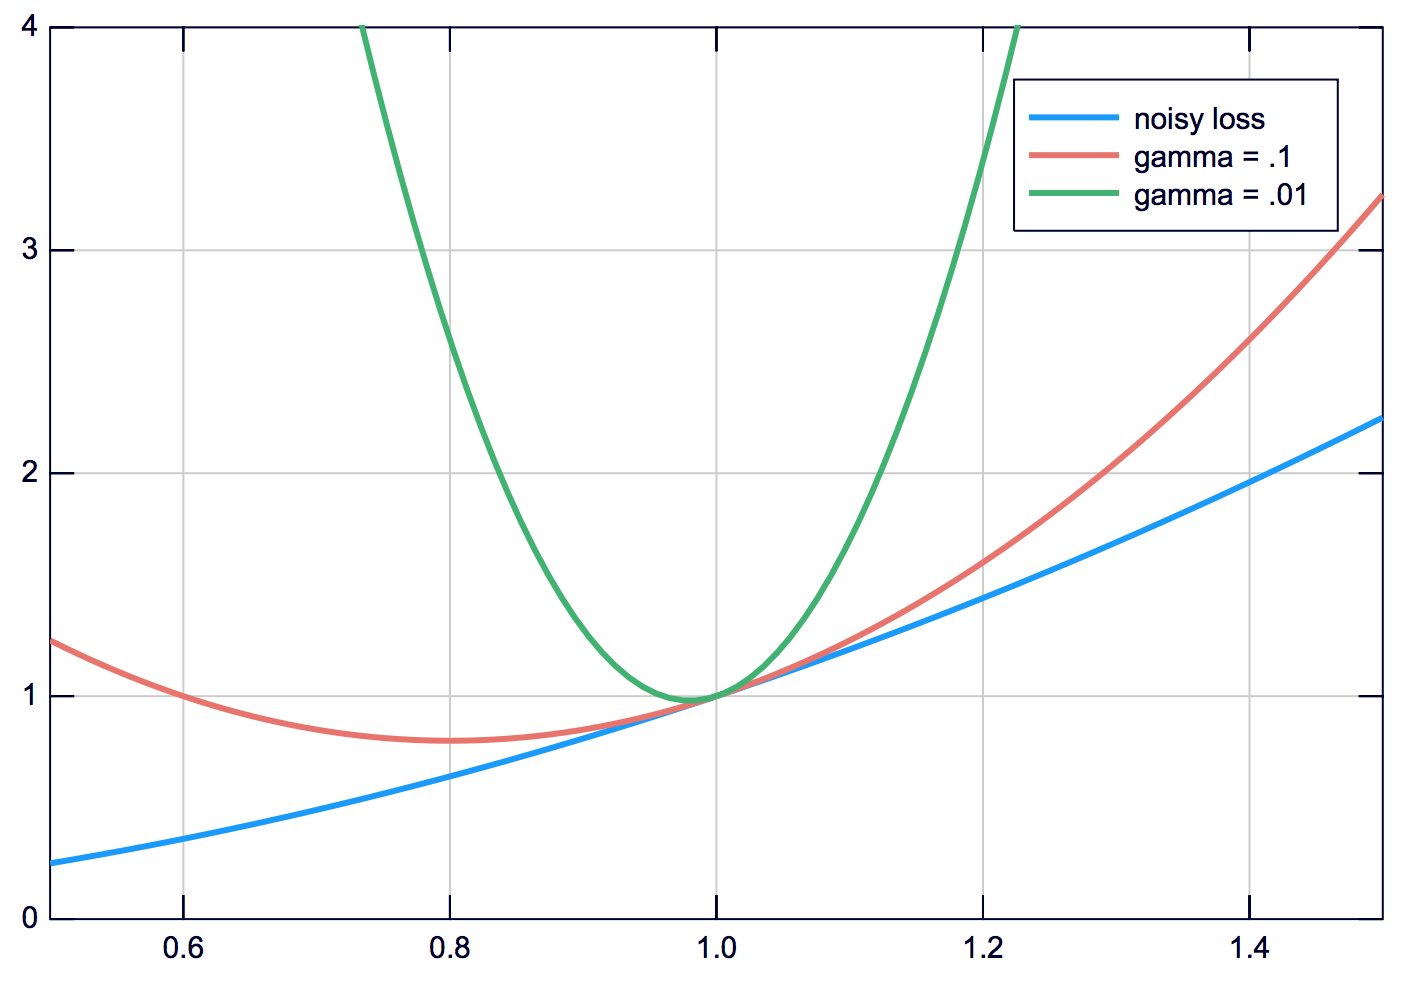
\includegraphics[width=.7\textwidth]{figures/quadraticupperbound.png}
    \end{figure}
  \end{itemize}
\end{frame}
\begin{frame}
  \begin{itemize}
    \item Majorizations get worse over time ($\gamma_t \rightarrow 0$), forcing the parameter to remain near its current state
  \end{itemize}
  \begin{figure}
    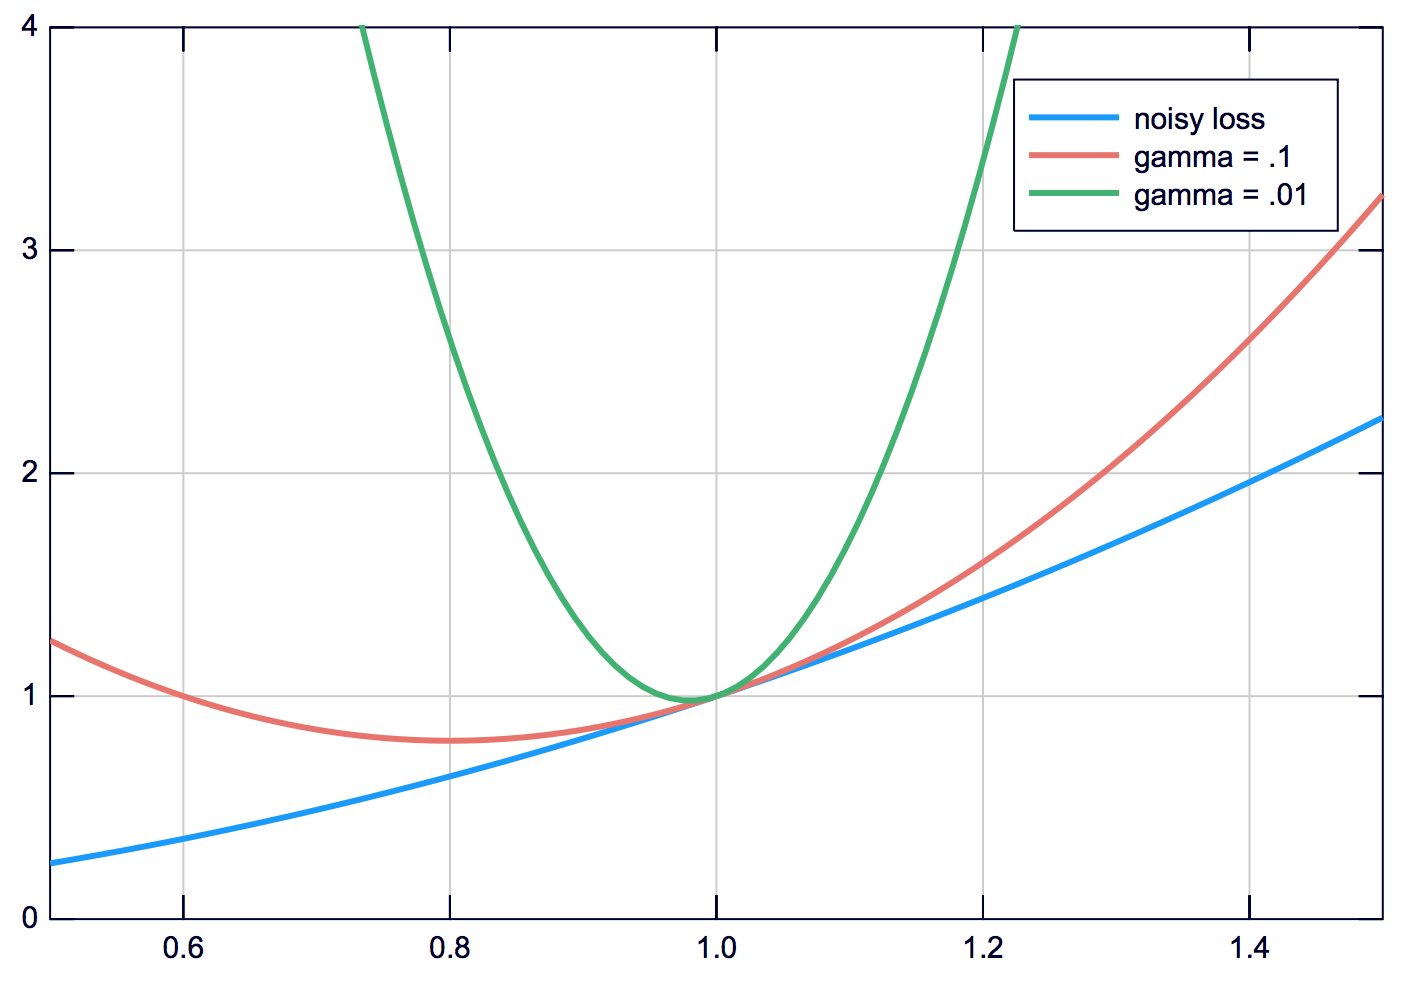
\includegraphics[width=.7\textwidth]{figures/quadraticupperbound.png}
  \end{figure}
\end{frame}



%%%%%%%%%%%%%%%%%%%%%%%%%%%%%%%%%%%%%%%%%%%%%%%%%%%%%%%%%%%%%%%%%%%%%%%%%%%%%%%%%%%%% Online MM
\section{Online MM}
\subsection{Setup}
\begin{frame}
  \frametitle{Online MM}
  \begin{itemize}
    \item Define an Online MM Algorithm as one which follows these steps for each observation/minibatch of data:
  \end{itemize}
  \begin{enumerate}
    \item observe $f_t(\bm\theta)$
    \item create majorization $h_t(\bm\theta)$
    \item Update surrogate objective function $Q_t(\bm\theta)$ with $h_t(\bm\theta)$
    \item $\iter{\bm\theta}{t+1} = argmin_{\bm\theta}Q_t(\bm\theta)$
  \end{enumerate}
\end{frame}
\begin{frame}
  \begin{itemize}
    \item Algorithms differ at step 3
    \item Ex: For SGD, $Q_t(\bm\theta) = h_t(\bm\theta)$, with conditions that $h_t$ is $m_t$-strongly convex (quadratic lower bound) and $m_t\rightarrow\infty$
  \end{itemize}
\end{frame}

\subsection{Online MM Types}
\begin{frame}
  \frametitle{Online MM Type 1}
  \begin{itemize}
    \item Rare case when there exists ``sufficient statistics'' for majorizing $\frac{1}{t}\sum_{\tau=1}^t f_\tau(\bm\theta)$ analytically
    \item Online majorization = offline majorization
  \end{itemize}
\end{frame}
\begin{frame}
  \frametitle{Online MM Type 2}
  \begin{itemize}
    \item $Q_t(\bm\theta) = (1 - \gamma_t)Q_{t-1}(\bm\theta) + \gamma_t h_t(\bm\theta)$
    \item Weighted average of surrogate objective and noisy majorization
  \end{itemize}
\end{frame}
\begin{frame}
  \frametitle{Online MM Type 3}
  \begin{itemize}
    \item $Q_t(\bm\theta) = h_t(\bm\theta)$, $h_t$ is $m_t$ strongly convex, $m_t\rightarrow\infty$
    \item SGD-like algorithms (ADAGRAD, ADAM)
  \end{itemize}
\end{frame}


%%%%%%%%%%%%%%%%%%%%%%%%%%%%%%%%%%%%%%%%%%%%%%%%%%%%%%%%%%%%%%%%%%%%%%%%%%%%%%%%%%%%% Simulations
\section{Simulation}
\subsection{Linear Regression}
\begin{frame}
  \begin{itemize}
    \item Learning Rate: $\gamma_t = t^{-r}, r\in[.5, .7, .9]$
  \end{itemize}
  \begin{figure}
    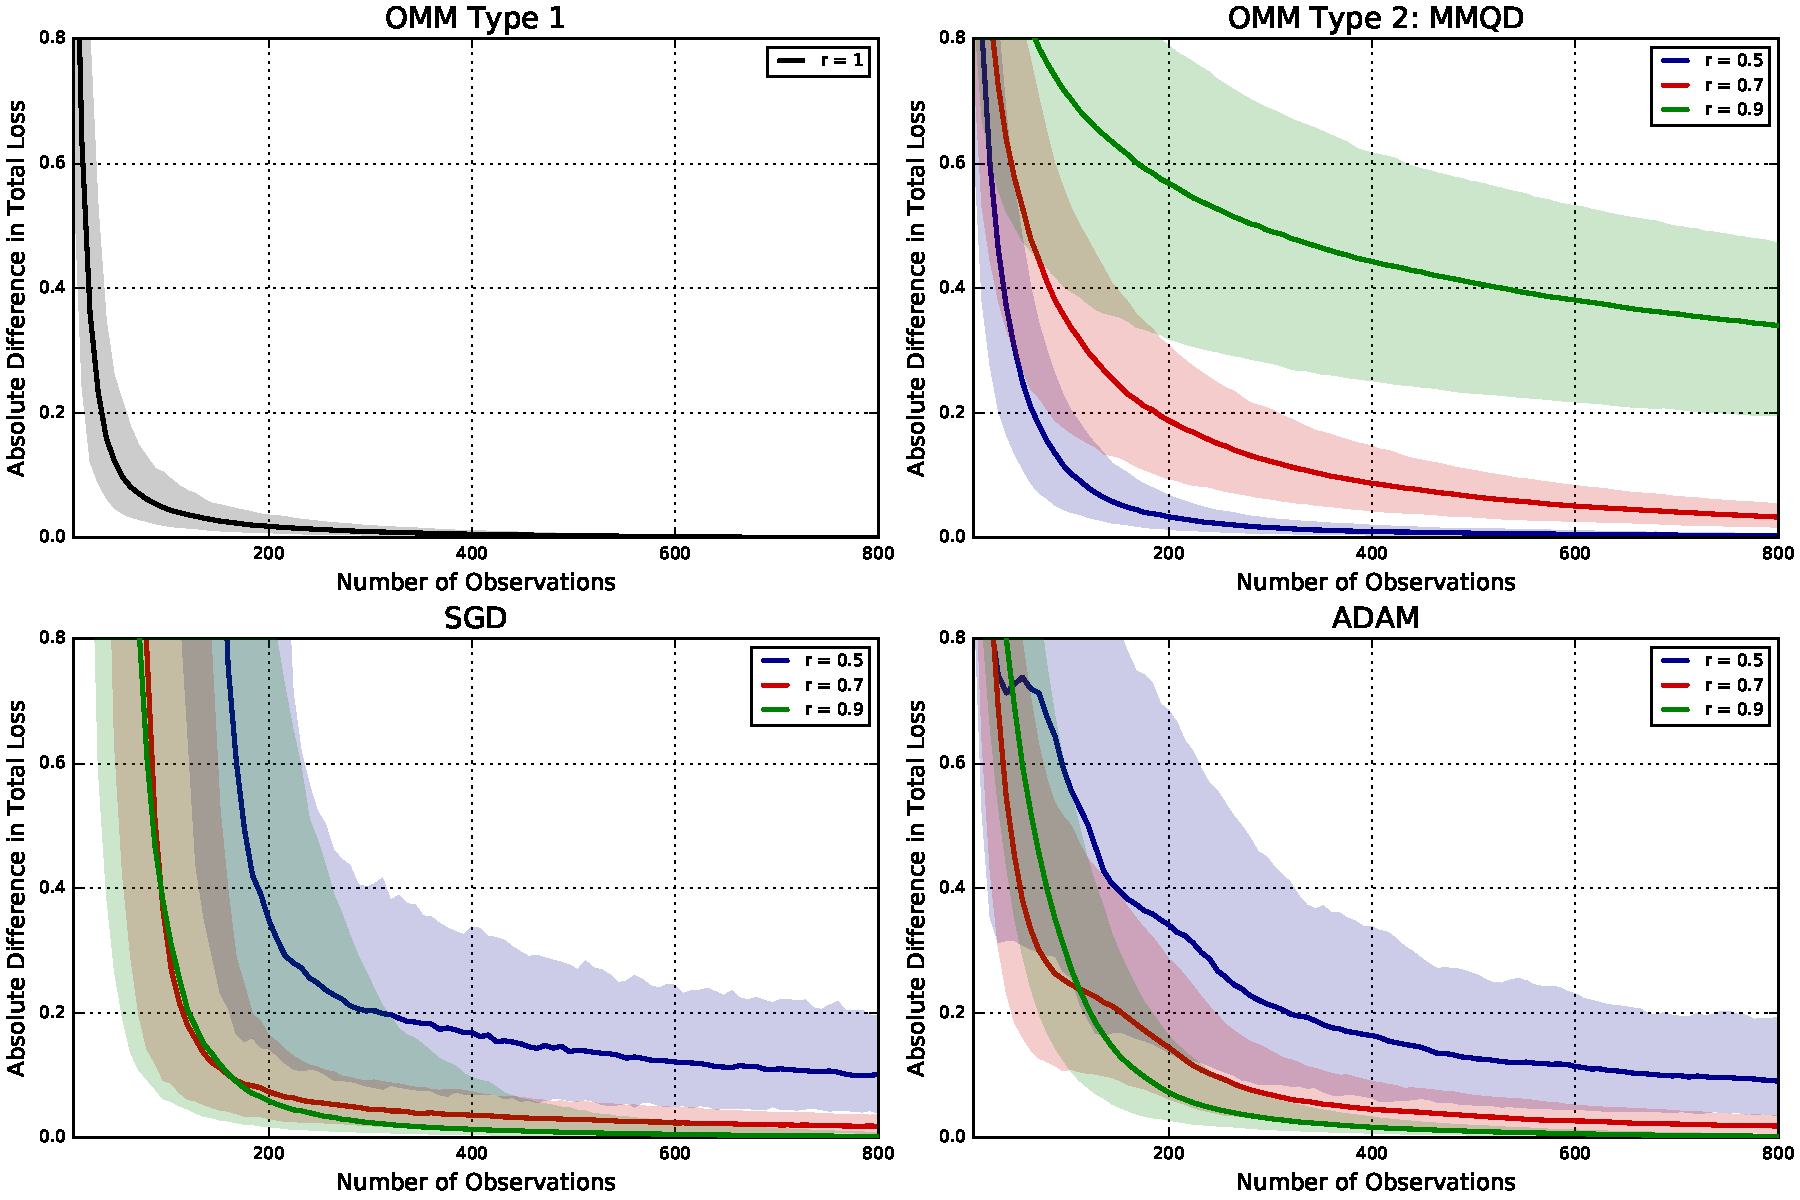
\includegraphics[width=\textwidth]{figures/linregmm_simulation.pdf}
  \end{figure}
\end{frame}

\subsection{Quantile Regression Regression}
\begin{frame}
  \begin{itemize}
    \item Learning Rate: $\gamma_t = t^{-r}, r\in[.5, .7, .9]$
  \end{itemize}
  \begin{figure}
    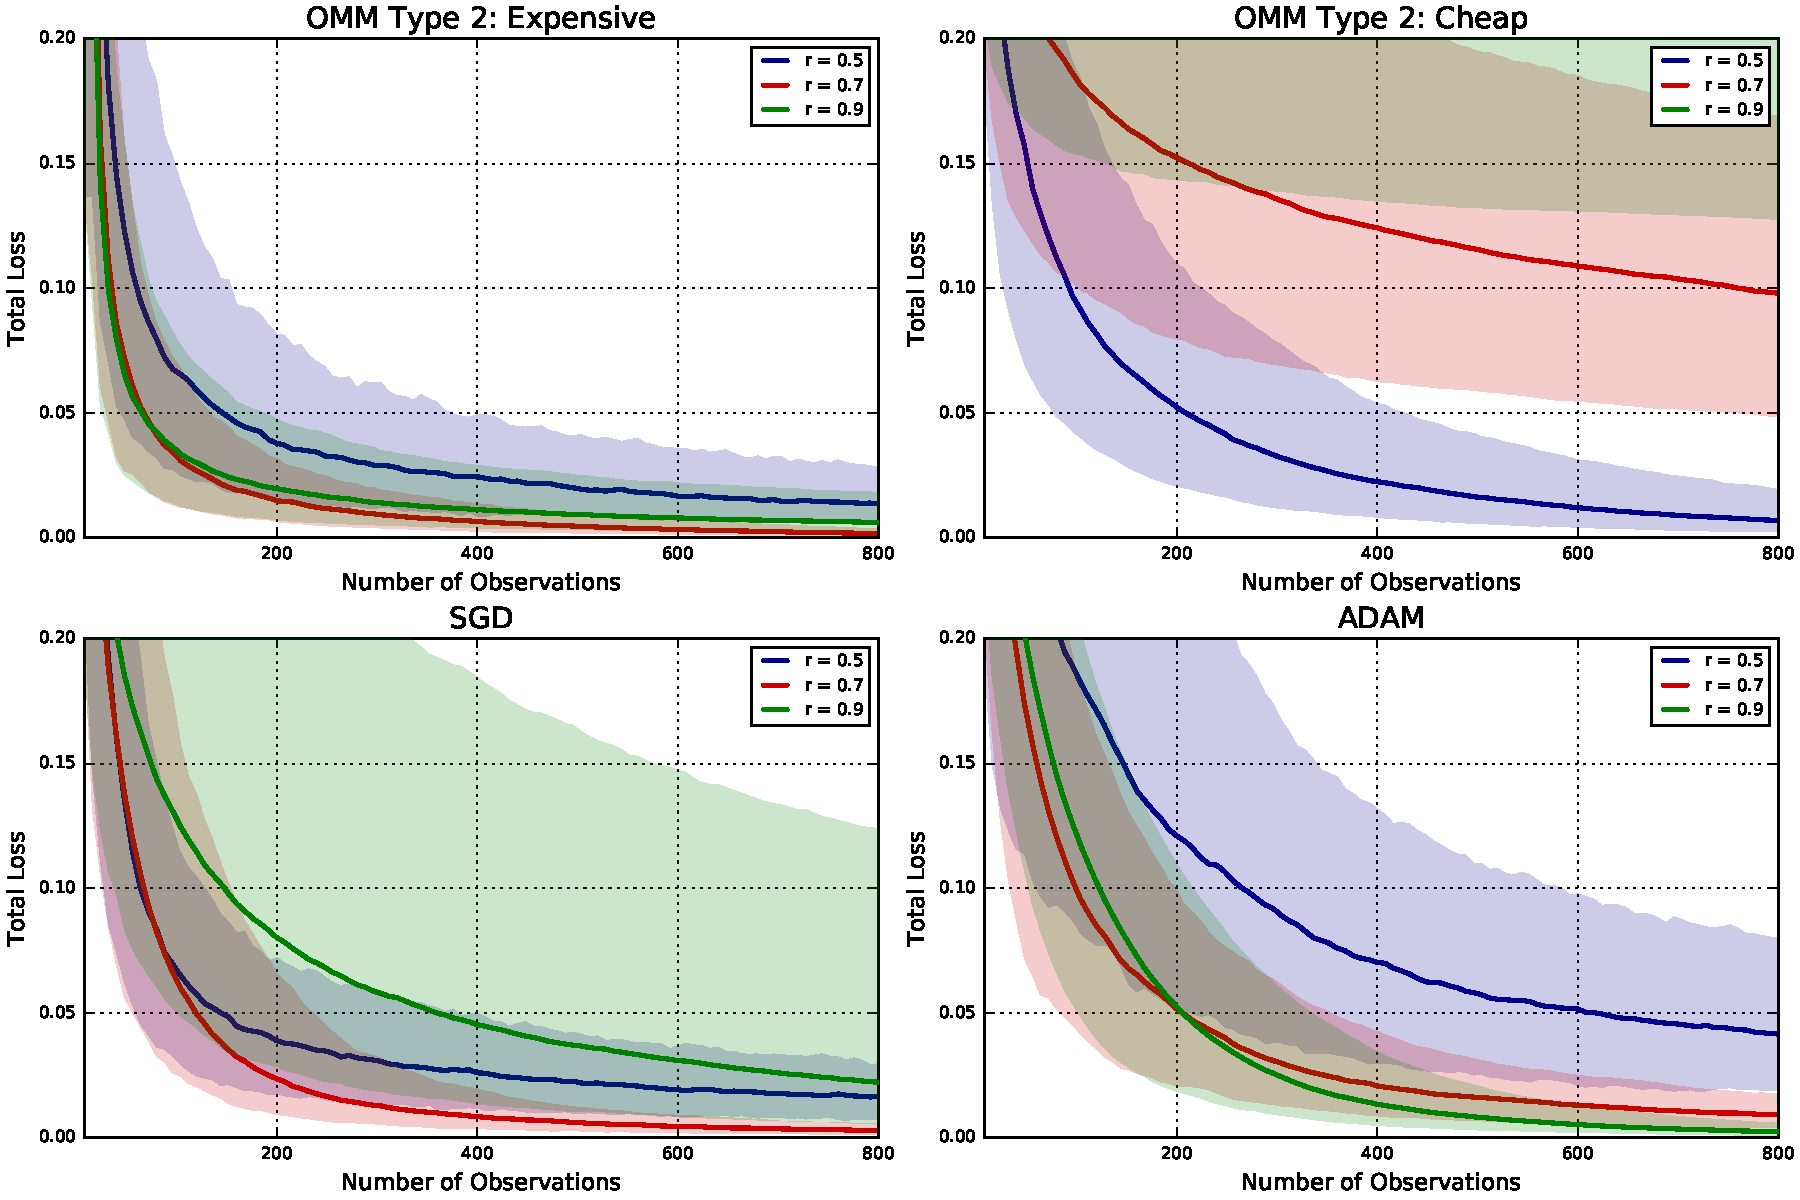
\includegraphics[width=\textwidth]{figures/quantreg_simulation.pdf}
  \end{figure}
\end{frame}

\subsection{Thanks}
\begin{frame}
  \frametitle{Thank You}
  \begin{itemize}
    \item Questions?
  \end{itemize}
\end{frame}


% %------------------------------------------------
%
% \begin{frame}
% \frametitle{Blocks of Highlighted Text}
% \begin{block}{Block 1}
% Lorem ipsum dolor sit amet, consectetur adipiscing elit. Integer lectus nisl, ultricies in feugiat rutrum, porttitor sit amet augue. Aliquam ut tortor mauris. Sed volutpat ante purus, quis accumsan dolor.
% \end{block}
%
% \begin{block}{Block 2}
% Pellentesque sed tellus purus. Class aptent taciti sociosqu ad litora torquent per conubia nostra, per inceptos himenaeos. Vestibulum quis magna at risus dictum tempor eu vitae velit.
% \end{block}
%
% \begin{block}{Block 3}
% Suspendisse tincidunt sagittis gravida. Curabitur condimentum, enim sed venenatis rutrum, ipsum neque consectetur orci, sed blandit justo nisi ac lacus.
% \end{block}
% \end{frame}
%
% %------------------------------------------------
%
% \begin{frame}
% \frametitle{Multiple Columns}
% \begin{columns}[c] % The "c" option specifies centered vertical alignment while the "t" option is used for top vertical alignment
%
% \column{.45\textwidth} % Left column and width
% \textbf{Heading}
% \begin{enumerate}
% \item Statement
% \item Explanation
% \item Example
% \end{enumerate}
%
% \column{.5\textwidth} % Right column and width
% Lorem ipsum dolor sit amet, consectetur adipiscing elit. Integer lectus nisl, ultricies in feugiat rutrum, porttitor sit amet augue. Aliquam ut tortor mauris. Sed volutpat ante purus, quis accumsan dolor.
%
% \end{columns}
% \end{frame}
%
%
%
% \begin{frame}
% \frametitle{Table}
% \begin{table}
% \begin{tabular}{l l l}
% \toprule
% \textbf{Treatments} & \textbf{Response 1} & \textbf{Response 2}\\
% \midrule
% Treatment 1 & 0.0003262 & 0.562 \\
% Treatment 2 & 0.0015681 & 0.910 \\
% Treatment 3 & 0.0009271 & 0.296 \\
% \bottomrule
% \end{tabular}
% \caption{Table caption}
% \end{table}
% \end{frame}






%------------------------------------------------

% \begin{frame}
% \frametitle{References}
% \footnotesize{
% \begin{thebibliography}{99} % Beamer does not support BibTeX so references must be inserted manually as below
% \bibitem[Smith, 2012]{p1} John Smith (2012)
% \newblock Title of the publication
% \newblock \emph{Journal Name} 12(3), 45 -- 678.
% \end{thebibliography}
% }
% \end{frame}



%----------------------------------------------------------------------------------------

\end{document}
